\documentclass[cn,11pt,chinese]{elegantbook}

\usepackage[all]{xy}
\usepackage{amsmath}
\usepackage{asymptote}
\usepackage{subfig}
\usepackage{graphicx}



\newcount\mycount
\def\cis{\,\text{cis}\,}
\def\intset{\operatorname{int}}
\def\diam{\operatorname{diam}}
\def\dist{\operatorname{dist}}
\def\ulim{\operatorname{u-lim}}
\def\cinfty{\mathbb{C}_{\infty}}
\def\sh{\operatorname{sh}}
\def\argsh{\operatorname{argsh}}
\def\ch{\operatorname{ch}}
\def\argch{\operatorname{argch}}
\def\real{\mathbb{R}}
\def\dsint{{\displaystyle\int}}

\numberwithin{equation}{section}


% title info
\title{微积分}
\subtitle{第一卷}

% bio info
\author{Tom. M. Apostol}

% extra info
\version{1.00}
\extrainfo{Wir m\"ussen wissen, wir werden wissen. (我们必须知道,我们必将知道) - David.Hilbert}
%\logo{logo.png}
\cover{cover.jpg}

\begin{document}


\maketitle

\chapter*{Preface}


\tableofcontents
\mainmatter
\hypersetup{pageanchor=true}

% add preface chapter here if needed

\chapter{Introduction}
\section{Historical Introduction}

\subsection{The two basic concepts of calculus}
The remarkable progress that has been made in science and technology during the last Century is due in large part to the development of mathematics. That branch of mathematics known as integral and differential calculus serves as a natural and powerful tool for attacking a variety of problems that arise in physics, astronomy, engineering, chemistry, geology, biology, and other fields including, rather recently, some of the social sciences.

To give the reader an idea of the many diffrent types of problems that can be treated by the methods of calculus, we list here a few sample questions selected from the exercises that occur in later chapters of this book.

With what speed should a rocket be fired upward so that it never returns to earth?What is the radius of the smallest circular disk that can cover every isosceles triangle of a given perimeter $L$? What volume of material is removed from a solid sphere of radius $2r$ if a hole of radius $r$ is drilled through the center? If a strain of bacteria grows at a rate proportional to the amount present and if the population doubles in one hour, by how much will it increase at the end of two hours? If a ten-pound force stretches an elastic spring one inch, how much work is required to stretch the spring one foot? 

These examples, chosen from various fields, illustrate some of the technical questions that can be answered by more or less routine applications of calculus.

Calculus is more than a technical tool --- it is a collection of fascinating and exciting ideas that have interested thinking men for centuries. These ideas have to do with speed, area, volume, rate of growth, continuity, tangent line, and other concepts from a variety of fields. Calculus forces us to stop and think carefully about the meanings  of these concepts. Another remarkable feature of the subject is its unifying power. Most of these ideas can be formulated so that they revolve around two rather specialized problems of a geometric nature. We turn now to a brief description of these problems.

Consider a curve $C$ which lies above a horizontal base line such as that shown in Figure 1.1. We assume this curve has the property that every vertical line intersects it once at most. The shaded portion of the figure consists of those points which lie below the curve $C$, above the horizontal base, and between two parallel vertical segments joining $C$ to the base. The first fundamental problem of calculus is this: To assign a number which measures the area of this shaded region.

Consider next a line drawn tangent to the curve, as shown in  Figure 1.1. The second fundamental problem may be stated as follow: To assign a number which measures the steepness of this line.

Basically, calculus has to do with the precise formulation and solution of these two special problems. It enables us to define the concepts of area and tangent line and to calculate the area of a given region or the steepness of a given tangent line. Untegral calculus deals with the problem of area and will be discussed in Chapter 1. Differential calculus deals with the problem of tangents and will be introduced in Chapter 4.

The study of calculus requires a certain mathematical background. The present chapter deals with this background material and is divided into four parts: Part 1 provides historical perspective; Part 2 discusses some notation and terminology from the mathematics sets; Part 3 deals with the real-number system; Part 4 treats mathematical induction and the summation notation. If the reader is acquainted with these topics, ha can proceed directly to the developmentof intergral calculus in Chapter 1. If not, he should become familiar with the material in the unstarred sections of this Introduction before proceeding to Chapter 1.

\subsection{Historical background}\label{section0010102}
The birth of integral calculus occurred more than 2000 years ago when the Greeks attemplted to determine areas by a process which they called the method of exhaustion. The essential ideas of this method are very simple and can be described briefly as follows: Given a region whose area is to be determined, we inscribe in it a polygonal region which approximates the given region and whose area we easily compute. Then we choose another polygonal region which gives a better approximation, and we continue the process, taking polygons with more and more sides in an attemplt to exhaust the given region. The method is illustrated for a semicircular region in Figure 1.2. It was used successfully by Archimedes (287 -212 B.C.) to find exact formulas for the area of a circle and a few other special figures.

The development of the method of exhaustion beyond the point to which Archimedes carried it has to wait nearly eighteen centuries until the use of algebraic symbols and techniques bacame a standard part of mathematics. The elementary algebra that is familiar to most high-school students today was completely unknown in Archimedes' time, and it would have been next to impossible to extend his method to any general class of regions without some convenient way of expressing rather lengthy calculations in a compact and simplified form.

A slow but revolutionary change in the development of mathematical notations began in the 16th century A.D. The cumbersome system of Roman numerals was gradually dispalced by the Hindu-Arabic characters used today, the symbols $+$ and $-$ were introduced for the first time, and the advantages of the decimal notation began to be recognized. During this same period, the brilliant successes of the Italian mathematicians Tartaglia, Cardano, and Ferrari in finding algebraic solutions of cubic and quartic equations stimulated a greatdeal of activity in mathematics and encouraged the growth and acceptance of a new superior algebraic language. With the widespread introduction of well-chosen algebraic symbols, interest was revived in the ancient method of exhaustion and a large number of fragmentary results were discovered in the 16th century by such pioneers as Cavalieri, Toricelli, Roberval, Fermat, Pascal, and Wallis.

Gradually the method of exhaustion was transformed into the subject now called integral calculus, a new and powerful discipline with a large variety of applications, not only to geometrical problems concerned with areas and volumes but also to problems in other sciences. This branch of mathematics, which retained some of the original features of the method of exhaustion, received its biggest impetus in the 17th century, largely due to the efforts of Isaac Newton (1642-1727) and Gottfried Leibniz (1646-1716), and its development continued well into the 19th century before the subject was put on a firm mathematical basis by such men as Augustin-Louis Cauchy (1789-1857) and Bernhard Riemann (1826-1866). Further refinements and extensions of the theory are still being carried out in contemporary mathematics.

\subsection{The method of exhaustion for the area of a parabolic segment}\label{section0010103}
Before we proceed to a systematic treatment of integral calculus, it will be instructive to apply the method of exhaustion directly to one of the special figures treated by Archimedes himself. The region in question is shown in Figure 1.3 and can be described as follows: If we choose an arbitrary point on the base of this figure and denote its distance from 0 by $x$, then the vertical distance from this point to the curve is $x^2$. In particular, if the length of the base itself is $b$, the altitude of the figure is $b^2$. The vertical distance from $x$ to curve is called the "ordinate" at $x$. The curve itself is an example of what is known as parabola. The region bounded by it and the two line segments is called a parabolic segment.

This figure may be enclosed in a rectangle of base $b$ and altitude $b^2$, as shown in Figure 1.3. Examination of the figure suggests that the area of the parabolic segment is less than half the area of the rectangle. Archimedes made the surprising discovery that the area of the parabolic segment is exactly one-third that of the rectangle; that id to say, $A = b^3/3$, where $A$ denotes the area of the parabolic segment. We shall show presently how to arrive at this result.

It should be pointed out that the parabolic segment in Figure 1.3 is not shown exactly as Archimedes drew it and the details that follow are not exactly the same as those used by him. Nevertheless, the essential ideas are those of Archimedes; what is presented here is the method of exhaustion in modern notation.

The method is simply this: We slice the figure into a number of strips and obtain two approximations to the region, one from below and one from above, by using two sets of rectangles as illustrated in Figure 1.4. (We use rectangles rather than arbitrary polygons to simplify the computations.) The area of the parabolic segment is larger than the total area of the inner rectangles but smaller than that of the outer rectangles.

If each strip is further subdivided to obtain a new approximation with a larger number of strips, the total area of the inner rectangles increases, whereas the total area of the outer rectangles decreases. Archimedes realized that an approximation to the area within any desired degree of accuracy could be obtained by simply taking enough strips.

Let us carry out the actual computations that are required in this case. For the cake of simplicity, we subdivide the base into $n$ equal parts, each of length $b/n$ (see Figure 1.5). The points of subdivision correspond to the following values of $x$:
\[
0, \frac{b}{n}, \frac{2b}{n}, \frac{3b}{n}, \cdots, \frac{(n-1)b}{n}, \frac{nb}{n} = b,
\]
A typical point of subdivision corresponds to $x=kb/n$, where $k$ takes the successive values $k=0,1,2,3,\cdots, n$. At each point $kb/n$ we construct the outer rectangle of altitude $(kb/n)^2$ as illustrated in Figure 1.5. The area of this rectangle is the product of its base and altitude and is equal to
\[
\left(\frac{b}{n}\right)\left(\frac{kb}{n}\right)^2 = \frac{b^3}{n^3}k^2.
\]
Let us denote by $S_n$ the sum of the areas of the outer rectangles. Then since the $k$th rectangle has area $(b^3/n^3)k^2$, we obtain the formula
\begin{equation}\label{equ001001}
S_n = \frac{b^3}{n^3}(1^2 + 2^2 + 3^2 + \cdots + n^2).
\end{equation}
In the same way we obtain a formula for the sum $s_n$ of all the inner rectangles:
\begin{equation}\label{equ001002}
s_n = \frac{b^3}{n^3}(1^2 + 2^2 + 3^2 + \cdots + (n-1)^2).
\end{equation}

This brings us to a very important stage in the calculation. Notice that the factor multiplying $b^3/n^3$ in Equation (\ref{equ001001}) is the sum of the squares of the first $n$ integers:
\[
1^2 + 2^2 + \cdots + n^2.
\]
[The corresponding factor in Equation (\ref{equ001002}) is similar except that the sum has only $n-1$ terms.] For a large value of $n$, the computation of this sum by direct addition of its terms is tedious and inconvenient. Fortunately there is an interesting identity which makes it possible to evaluate this sum in a simpler way, namely,
\begin{equation}\label{equ001003}
1^2 + 2^2 + \cdots + n^2 = \frac{n^3}{3} + \frac{n^2}{2} + \frac{n}{6}.
\end{equation}
This identity is valid for every integer $n \ge 1$ and can be proved as follows: Start with the formula $(k+1)^3= k^3 + 3k^2 + 3k + 1$ and rewrite it in the form
\[
3k^2 + 3k + 1 = (k+1)^3 - k^3. 
\]
Taking $k=1,2,\cdots, n-1$, we get $n-1$ formulas
\[
\begin{aligned}
3 \cdot 1^2 + 3 \cdot 1 + 1 &= 2^3 - 1^3\\
3 \cdot 2^2 + 3 \cdot 2 + 1 &= 3^3 - 2^3\\
\vdots&\\
3(n-1)^2 + 3(n-1) + 1 &= n^3 - (n-1)^3.
\end{aligned}
\]
When we add these formulas, all the terms on the right cancel except two and we obtain
\[
3[1^2+2^2+\cdots+(n-1)^2] + 3[1+2+\cdots+(n-1)] + (n-1) = n^3 - 1^3.
\]
The second sum on the left is the sum of terms in an arithmetic progression and it simplifies to $\frac{1}{2}n(n-1)$. Therefore this last equation gives us
\begin{equation}\label{equ001004}
1^2 + 2^2 + \cdots + (n-1)^2 = \frac{n^3}{3} - \frac{n^2}{2} + \frac{n}{6}.
\end{equation}
Adding $n^2$ to both members, we obtain (\ref{equ001003}).

For our purposes, we do not need the exact expressions given in the right-hand members of (\ref{equ001003}) and (\ref{equ001004}). All we need are the two inequalities
\begin{equation}\label{equ001005}
1^2 + 2^2 + \cdots + (n-1)^2 < \frac{n^3}{3} < 1^2 + 2^2 + \cdots + n^2
\end{equation}
which are valid for every integer $n \ge 1$. These inequalities can be deduced easily as consequences of (\ref{equ001003}) and (\ref{equ001004}), or they can be proved directly by induction. (A proof by induction is given in Section \ref{section0010401})

If we multiply both inequalities in (\ref{equ001005}) by $b^3/n^3$ and make use of (\ref{equ001001}) and (\ref{equ001002}), we obtain 
\begin{equation}\label{equ001006}
s_n < \frac{b^3}{3} < S_n
\end{equation}
for every $n$. The inequalities in (\ref{equ001006}) tell us that $b^3/3$ is a number which lies between $s_n$ and $S_n$ for every $n$. We will now prove that $b^3/3$ is the only number which has this property. In other words, we assert that if $A$ is any number which satisfies the inequalities
\begin{equation}\label{equ001007}
s_n < A < S_n
\end{equation}
for every positive integer $n$, then $A = B^3/3$. It is because of this fact that Archimedes concluded that the area of the parabolic segment is $b^3/3$.

To prove that $A = b^3/3$, we use the inequalities in (\ref{equ001005}) once more. Adding $n^2$ to both sides of the leftmost inequality in (\ref{equ001005}), we obtain
\[
1^2 + 2^2 + \cdots + n^2 < \frac{n^3}{3}+ n^2.
\]
Multiplying this by $b^3/n^3$ and using (\ref{equ001001}), we find
\begin{equation}\label{equ001008}
S_n < \frac{b^3}{3} + \frac{b^3}{n}.
\end{equation}
Similarly, by subtracting $n^2$ from both sides of the rightmost inequality in (\ref{equ001005}) and multiplying by $b^3/n^3$, we are led to the inequality
\begin{equation}\label{equ001009}
\frac{b^3}{3} - \frac{b^3}{n} < s_n.
\end{equation}
Therefore, any number $A$ satisfying (\ref{equ001007}) must also satisfy
\begin{equation}\label{equ001010}
\frac{b^3}{3} - \frac{b^3}{n} < A < \frac{b^3}{3} + \frac{b^3}{n}
\end{equation}
for every integer $n \ge 1$. Now there are only three possibilities:
\[
A > \frac{b^3}{3}, \quad A < \frac{b^3}{3}, \quad A = \frac{b^3}{3}.
\]
If we show that each of the first two leads to a contradiction, then we must have $A = b^3/3$, since, in the manner of Sherlock Holmes, this exhausts all the possibilities.

Suppose the inequality $A > b^3/3$ were true. From the second inequality in (\ref{equ001010}) we obtain
\begin{equation}\label{equ001011}
A - \frac{b^3}{3} < \frac{b^3}{n}
\end{equation}
for every integer $n \ge 1$. Since $A - b^3/3$ is positive, we may divide both sides of (\ref{equ001011}) by $A - b^3/3$ and then multiply by $n$ to obtain the equivalent statement
\[
n < \frac{b^3}{A - b^3/3}
\]
for every $n$. But this inequality is obviously false when $n > b^3/(A - b^3/3)$. Hence the inequality $A > b^3/3$ leads to a contradiction. By a similar argument,we can show that the inequality $A < b^3/3$ also leads to a contradiction, and therefore we must have $A = b^3/3$, as asserted.

\subsection{Exercises}
\begin{enumerate}
\item[1.] (a) Modify the region in Figure 1.3 by assuming that the ordinate at each $x$ is $2x^2$ instead of $x^2$. Draw the new figure. Check through the principal steps in the foregoing section and find what effect this has on the calculation of the area. Do the same if the ordinate at each $x$ is (b) $3x^2$, (c) $\frac{1}{4}x^2$, (d) $2x^2+1$, (e) $ax^2+c$.

\item[2.] Modify the region in Figure 1.3 by assuming that the ordinate at each $x$ is $x^3$ instead of $x^2$. Draw the new figure.

(a) Use a construction similar to that illustrated in Figure 1.5 and show that the outer and inner sums $S_n$ and $s_n$ are given by
\[
S_n = \frac{b^4}{n^4}(1^3+2^2+\cdots+n^3),\quad s_n = \frac{b^4}{n^4}[1^3+2^3+\cdots + (n-1)^3].
\]

(b) Use the inequalities (which can be proved by mathematical induction; see Section \ref{section0010402})
\begin{equation}\label{equ001012}
1^3 + 2^3 + \cdots + (n-1)^3 < \frac{n^4}{4} < 1^3 + 2^3 + \cdots + n^3
\end{equation}
to show that $s_n < b^4/4 < S_n$ for every $n$, and prove that $b^4/4$ is the only number which lies between $s_n$ and $S_n$ for every $n$.

(c) What number takes the place of $b^4/4$ if the ordinate at each $x$ is $ax^3+c$?

\item[3.] The inequalities (\ref{equ001005}) and (\ref{equ001012}) are special cases of the more general inequalities
\begin{equation}\label{equ001013}
1^k + 2^k + \cdots + (n-1)^k < \frac{n^{k+1}}{k+1} < 1^k + 2^k + \cdots + n^k
\end{equation}
that are valid for every $n \ge 1$ and every integer $k \ge 1$. Assume the validity of (\ref{equ001013}) and generalize the results of Exercise 2.
\end{enumerate}

\subsection{A critical analysis of Archimedes' method}
From calculations similar to those in Section 1.3, Archimedes concluded that the area of the parabolic segment in question is $b^3/3$. This fact was generally accepted as a mathematical theorem for nearly 2000 years before it was realized that one must re-examine the result from a more critical point of view. To understand why anyone would question the validity of Archimedes' conclusion, it is necessary to know something about the important changes that have taken place in the recent history of mathematics.

Every branch of knowledge is a collection of ideas described by means of words and symbols, and one cannot understand these ideas unless one knows the exact meanings of the words and symbols that are used. Certain branches of knowledge, known as deductive systems, are different from others in that a number of "undefined" concepts are chosen in advance and all other concepts in the system are defined in terms of these. Certain statements about these undefined concepts are taken as axioms or postulates and other statements that can be deduced from the axioms are called theorems. The most familiar example of a deductive system is the Euclidean theory of elementary geometry that has been studied by well-educated men since the time of the ancient Greeks.

The spirit of early Greek mathematics, with its emphasis on the theoretical and postulational approach to geometry as presented in Euclid's Elements, dominated the thinking of mathematicians until the time of the Renaissance. A new and vigorous phase in the development of mathematics began with the advent of algebra in the 16th century, and the next 300 years witnessed a flood of important discoveries. Conspicuously absent from this period was the logically precise reasoning of the deductive method with its use of axioms, definitions, and theorems. Instead, the pioneers in the 16th, 17th, and 18th centuries resorted to a curious blend of deductive reasoning combined with intuition, pure guesswork, and mysticism, and it is not surprising to find that some of their was later shown to be incorrect. However, a surprisingly large number of important discoveries emerged from this era, and a great deal of the work has survived the test of history --- a tribute to the unusual skill and ingenuity of these pioneers.

As the flood of new discoveries began to recede, a new and more critical period emerged. Little by little, mathematicians felt forced to return to the classical ideas of the deductive method in an attempt to put the new mathematics on a firm foundation. This phase of the development, which began early in the 19th century and has continued to the present day, has resulted in a degree of logical purity and abstraction that has surpassed all the traditions of Greek science. At the same time, it has brought about a clearer understanding of the foundations of not only calculus but of all of mathematics.

There are many ways to develop calculus as a deductive system. One possible approach is to take the real numbers as the undefined objects. Some of the rules governing the operations on real numbers may then be taken as axioms. One such set of axioms is listed in Part 3 of this Introduction. New concepts, such as integral, limits, continuity, derivative, must then be defined in terms of real numbers. Properties of these concepts are then deduced as theorems that follow from the axioms.

Looked at as part of the deductive system of calculus, Archimedes' result about the area of a parabolic segment cannot be accepted as a theorem until a satisfactory definition of a area is given first. It is not clear whether Archimedes has ever formulated a precise definition of what he meant by area. He seems to have taken it for granted that every region has an area associated with it. On this assumption he then set out to calculate areas of particular regions. In his calculations he made use of certain facts about area that cannot be proved until we know what is meant by area. For instance, he assumed that if one region lies inside another, the area of the smaller region cannot exceed that of the larger region. Also, if a region is decomposed into two or more parts, the sum of the areas of the individual parts is equal to the area of the whole region. All these are properties we would like area to possess, and we shall insist that any definition of area should imply these properties. It is quite possible that Archimedes himself may have taken area to be an undefined concept and then used the properties we just mentioned as axioms about area.

Today we consider the work of Archimedes as being important not so much because it helps us to compute areas of particular figures, but rather because it suggests a reasonable way to define the concept of area for more or less arbitrary figures. As it turns out, the method of Archimedes suggests as way to define a much more general concept known as the integral. The integral, in turn, is used compute not only area but also quantities such as arc length, volume, work and others.

If we look ahead and make use if the terminology of integral calculus, the result of the calculation carried out in Section {\ref{section0010103}} for the parabolic segment is often stated as follows: 
\centerline{"The integral of $x^2$ from $0$ to $b$ is $b^3/3$."}
It is written symbolically as 
\[
\int_{0}^{b}{x^2dx} = \frac{b^3}{3}.
\]
The symbol $\int$ (an elongated $S$) is called an integral sign, and it was introduced by Leibniz in 1675. The process which produces the number $b^3/3$ is called integration. The numbers $0$ and $b$ which are attached to the integral sign are referred to as the limits of integration. The symbol $\int_{0}^{b}{x^2dx}$ must be regarded as a whole. Its definition will treat it as such, just as the dictionary describes the word "lapidate" without reference to "lap,""id," or "ate."

Leibniz' symbol for the integral was readily accepted by many early mathematicians because they linked to think of integration as a kind of "summation process" which enabled them to add together infinitely many "infinitesimally small quantities." For example, the area of the parabolic segment was conceived of as a sum of infinitely many infinitesimally thin rectangles of height $x^2$ and base $dx$. The integral sign represented the process of adding the areas of all these thin rectangles. This kind of thinking is suggestive and often very helpful, but it is not easy to assign a precise meaning to the idea of an "infinitesimally small quantity." Today the integral is defined in terms of the notion of real number without using ideas like "inifitesimals." This definition is given in Chapter \ref{chapter002}.


\subsection{The approach to calculus to be used in this book}
A thorough and complete treatment of either integral or differential calculus depends ultimately on a careful study of the real number system. This study in itself, when carried out in full, is an intersting but somewhat lengthy program that requires a small volume for its complete exposition. The approach in this book is to begin with the real numbers as undefined objects and simply to list a number of fundamental properties of real numbers which we shall take as axioms. These axioms and some of the simplest theorems that can be deduced from them are discussed in Part \ref{section00103} of this chapter.

Most of the properties of real numbers discussed here are probably familiar to the reader from his study of elementary algebra. However, there are a few properties of real numbers that do not ordinarily come into consideration in elementary algebra but which play an important role in the calculus. These properties stem from the so-called least-upper-bound axiom (also known as the completeness or continuity axiom) which is dealt with here in some detail. The reader may wish to study Part \ref{section00103} before proceeding with the main body of the text, or he may postpone reading this material until later when he reaches those parts of the theory that make use of least-upper-bound properties. Material in the text that depends in the least-upper-bound axiom will be clearly indicated.

To develop calculus as a complete, formal mathematical theory, it would be necessary to state, in addition to the axioms for the real number system, a list of the various "methods of proof" which would be permitted for the purpose of deducing theorems from the axioms. Every statement in the theory would then have o be justified either as an "established law"(that is, an axiom, a definition, or a previously proved theorem) or as the result of applying one of the acceptable methods of proof to an established law. A program of this sort would be extremely long and tedious and would add very little to a beginner's understanding of the subject. Fortunately, it is not necessary to proceed in this fashion in order to get a good understanding and a good working knowledge of calculus. In this book the subject is introduced in an informal way, and ample use is made of geometric intuition whenever it is convenient to do so. At the same time, the discussion proceeds in a manner that is consistent with modern standards of precision and clarity of thought. All the important theorems of the subject are explicitly stated and rigorously proved.

To avoid interrupting the principal flow of ideas, some of the proofs appear in separate starred sections. For the same reason, some of the chapters are accompanied by supplemenatry material in which certain important topics related to calculus are dealt with in detail. Some of these are also starred to indicate that they may be omitted or postponed without disrupting the continuity of the presentation. The extent to which the starred sections are taken up or not will depend partly on the reader's background and skill and partly on the depth of his interests. A person who is interested primarily in the basic techniques may skip the starred sections. Those who wish a more thorough course in calculus, including theory as well as technique, should read some of the starred sections.



\section{Some Basic Concepts of the Theory of Sets}\label{section00102}

\subsection{Introduction to set theory}
In discussing any branch of mathematics, be it analysis, algebra, or geometry, it is helpful to use the notation and terminology of set theory. This subject, which was developed by Boole and Cantor\footnote{George Boole(1815 - 1864) was an English mathematician and ligician. His book, An Investigation of the Laws of Thought. published in 1854, marked the creation of the first workable system of symbolic logic. Georg F. L. P. Cantor (1845-1918) and his school created the modern theory of sets during the period 1874-1895.} in the latter part of the 19th century, has had a profound influence on the development of mathematics in the 20th century. It has unified many seemingly disconnected ideas and has helped to reduce many mathematical concepts to their logical foundations in an elegant and systematic way.  A thorough treatment of the theory of sets would require a lengthy discussion which we regard as outside the scope of this book. Fortunately, the basic notions are few in number, and it is possible to develop a working knowledge of the methods and ideas of set theory through an informal discussion. Actually, we shall discuss not so much a new theory as an agreement about the precise termonology that we wish to apply to more  or less familiar ideas.

In mathematics, the word "set" is used to represent a collection of objects viewed as a single entity. The collections called to mind by such nouns as "flock," "tribe," "crowd," "team," and "electorate" are all examples of sets. The individual objects in the collection are called elements or members of the set, and they are said to belong to or be contained in the set. The set, in turn, is said to contain or be composed of its elements.

We shall be interested primarily in sets of mathematical objects: sets of numbers, sets of curves, sets of geometric figures, and so on. In many applications it is convenient to deal with sets in which nothing special is assumed about the nature of the individual objects in the collection. These are called abstract sets. Abstract set theory has been developed to deal with such collections of arbitrary objects, and from this generality the theory derives its power.


\subsection{Notations for designating sets}
Sets usually are denoted by capital letters: $A,B,C,\cdots,X,Y,Z$; elements are designated by lower-case letters: $a,b,c,\cdots,x,y,z$. We use the special notation
\[
x \in S
\]
to mean that "$x$ is an element of $S$" or "$x$ belongs to $S$." If $x$ does not belong to $S$, we write $x \notin S$. When convenient, we shall designate sets by displaying the elements in braces; for example, the set of positive even integers less than 10 is denoted as $\{2, 4, 6, \cdots\}$, the three dots taking the place of "and so on." The dots are used only when the meaning of "and so on" is clear. The method of listing the members of a set within braces is sometimes referred to as the roster notation.

The first basic concept that relates one set to another is equality of sets: 
\begin{definition}{DEFINITION OF SET EQUALITY}{def0010201}
Two sets $A$ and $B$ are said to be equal (or identical) if they consist of exactly the same elements, in which case we write $A = B$. If one of the sets contains an element not in the other, we say the sets are unequal and we write $A \neq B$.
\end{definition}

\begin{example}
According to this definition, the two sets $\{2,4,6,8\}$ and $\{2,8,6,4\}$ are equal since they both consist of the four integers $2,4,6$, and 8. Thus, when we use the roster notation to describe a set, the order in which the elements appears is irrelevant.
\end{example}

\begin{example}
The sets $\{2,4,6,8\}$ and $\{2,2,4,4,6,8\}$ are equal even though, in the second set, each of the elements $2$ and $4$ is listed twice. Both sets contains the four elements 2,4,6,8 and no others; therefore, the definition requires that we call these sets equal. This example shows that we do not insist that the objects listed in the roster notation be distinct. A similar example is the set of letters in the word Mississippi, which is equal to the set \{M, i, s, p\}, consisting of the four distinct letters M, i, s, and p.
\end{example}


\subsection{Subsets}
From a given set $S$ we may form new sets, called subsets of $S$. For example, the set consisting of those positive integers less tha 10 which are divisible by 4 (the set $\{4, 8\}$) is a subset of the set of all even integers less than 10. In general, we have the following definition.
\begin{definition}{DEFINITION OF A SUBSET}{def0010202}
A set $A$ is said to be a subset of a set $B$, and we write 
\[
A \subset B,
\]
whenever every element of $A$ also belongs to $B$. We also say that $A$ is contained in $B$ or that $B$ contains $A$. The relation $\subset$ is referred to as set inclusion.
\end{definition}

The statement $A \subset B$ does not rule out the possibility that $B \subset A$. In fact, we may have both $A \subset B$ and $B \subset A$, but this happens only if $A$ and $B$ have the same elements. In other words,
\[
A = B\quad \text{if and only if} \quad A \subset B \text{ and } B \subset A.
\]
This theorem is an immediate consequence of the foregoing definitions of equality and inclusion. If $A \subset B$ but $A \neq B$, then we say that $A$ is a proper subset of $B$; we indicate this by writing $A \subsetneqq B$.

In all our applications of set theory, we have a fixed set $S$ given in advance, and we are concerned only with subsets of this given set. The underlying set $S$ may vary from one application to another; it will be referred to as the universal set of each particular discourse. The notation 
\[
\{x | x \in S \text{ and } x \text{ satisfies } P\}
\]
will designate the set


\subsection{Unions, intersections, complements}



\subsection{Exercises}


\section{A Set of Axioms for the Real-Number System}\label{section00103}


\subsection{Introduction}


\subsection{The field axioms}


\subsection{Exercises}


\subsection{The order axioms}


\subsection{Exercises}


\subsection{Integers and rational numbers}



\subsection{Geometric interpretation of real numbers as points on a line}


\subsection{Upper bound of a set, maximum element, least upper bound (supremum)}


\subsection{The least-upper-bound axiom (completeness axiom)}



\section{Mathematical Induction, Summation Notation, and Related Topics}\label{section00104}

\subsection{An example of a proof by mathematical induction}\label{section0010401}



\subsection{The principle of mathematical induction}\label{section0010402}


\chapter{The Concepts of Integral Calculus}\label{chapter002}








% \bibliographystyle{plain}
\bibliography{mathreference}
\appendix
% h
\chapter{Tikz绘制的一些图形}
\begin{center}
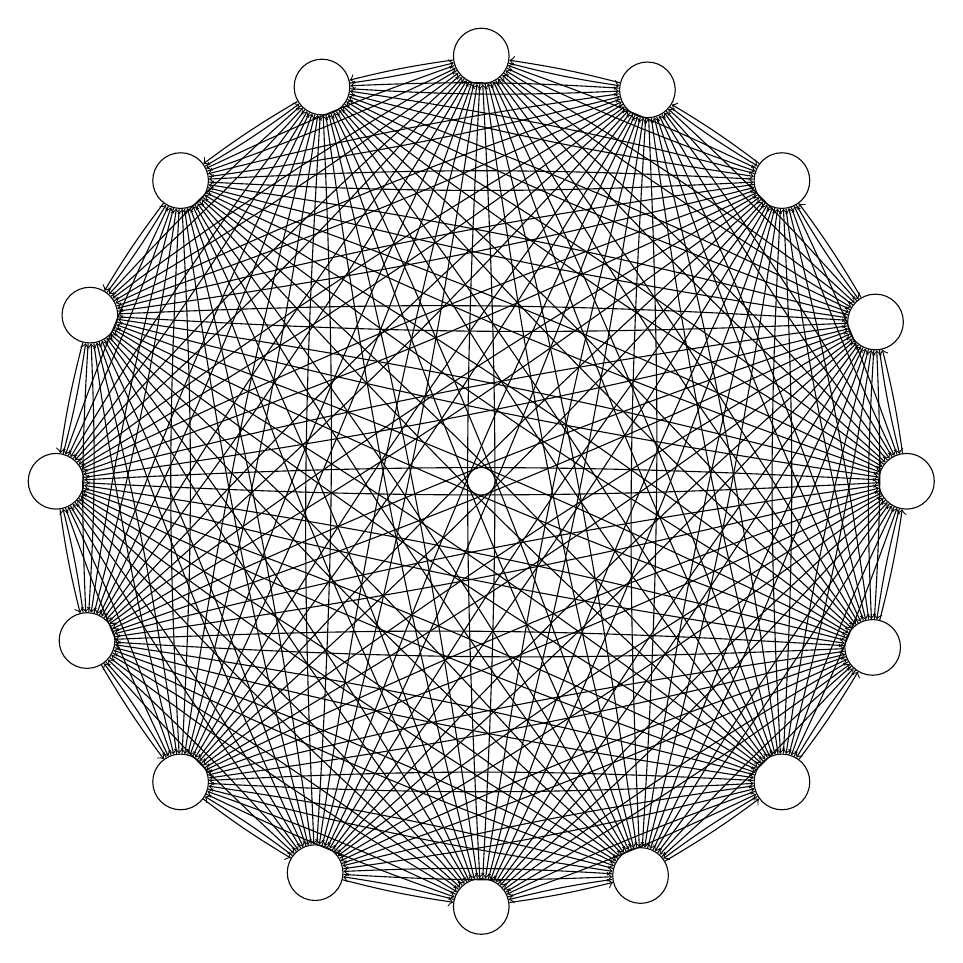
\begin{tikzpicture}[transform shape]
  %the multiplication with floats is not possible. Thus I split the loop in two.
  \foreach \number in {1,...,8}{
      % Computer angle:
        \mycount=\number
        \advance\mycount by -1
  \multiply\mycount by 45
        \advance\mycount by 0
      \node[draw,circle,inner sep=0.25cm] (N-\number) at (\the\mycount:5.4cm) {};
    }
  \foreach \number in {9,...,16}{
      % Computer angle:
        \mycount=\number
        \advance\mycount by -1
  \multiply\mycount by 45
        \advance\mycount by 22.5
      \node[draw,circle,inner sep=0.25cm] (N-\number) at (\the\mycount:5.4cm) {};
    }
  \foreach \number in {1,...,15}{
        \mycount=\number
        \advance\mycount by 1
  \foreach \numbera in {\the\mycount,...,16}{
    \path (N-\number) edge[->,bend right=3] (N-\numbera)  edge[<-,bend
      left=3] (N-\numbera);
  }
}
\end{tikzpicture}


\begin{tikzpicture}
 \definecolor{r1}{RGB}{0,129,188}
 \definecolor{r2}{RGB}{252,177,49}
 \definecolor{r3}{RGB}{35,34,35}
 \definecolor{r4}{RGB}{0,157,87}
 \definecolor{r5}{RGB}{238,50,78}
 \begin{scope}
   \clip (-6,2) rectangle (6,-.9);
   \foreach \col/\xp/\yp in {
     r5/4/0, r4/2/-1.8, r3/0/0,
     r2/-2/-1.8, r1/-4/0
   } {
     \path[draw=white,line width=.08cm,
     fill=\col,even odd rule]
     (\xp, \yp) circle (1.9cm)
     (\xp, \yp) circle (1.5cm);
   }
 \end{scope}
 \begin{scope}
   \clip (-6,-.9) rectangle (6,-3.8);
   \foreach \col/\xp/\yp in {
     r1/-4/0, r2/-2/-1.8, r3/0/0,
     r4/2/-1.8, r5/4/0
   } {
     \path[draw=white,line width=.08cm,
     fill=\col,even odd rule]
     (\xp, \yp) circle (1.9cm)
     (\xp, \yp) circle (1.5cm);
   }
 \end{scope}
\end{tikzpicture}


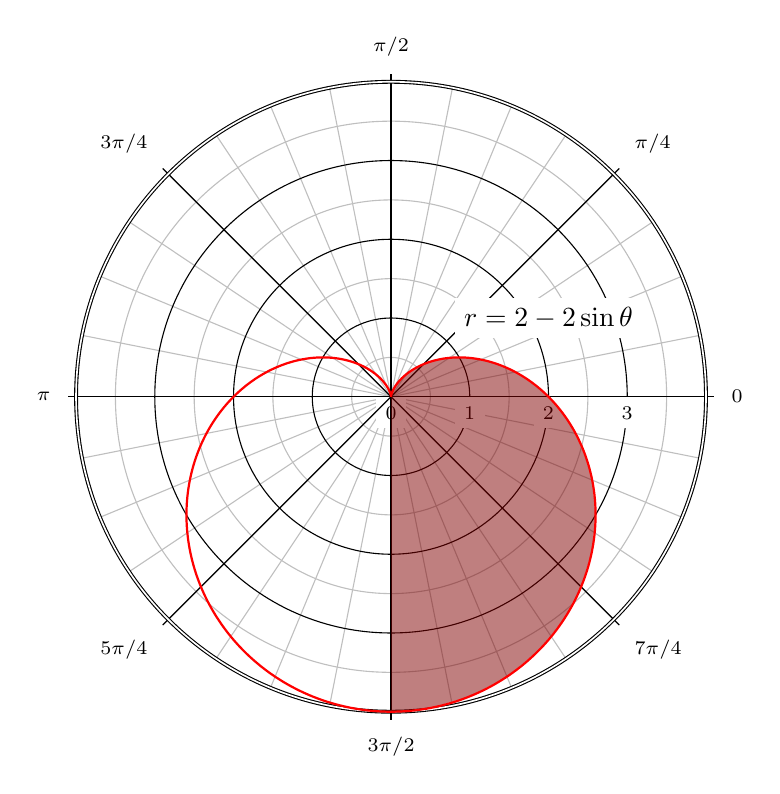
\begin{tikzpicture}[>=latex]

% Draw the lines at multiples of pi/12
\foreach \ang in {0,...,31} {
  \draw [lightgray] (0,0) -- (\ang * 180 / 16:4);
}

% Concentric circles and radius labels
\foreach \s in {0, 1, 2, 3} {
  \draw [lightgray] (0,0) circle (\s + 0.5);
  \draw (0,0) circle (\s);
  \node [fill=white] at (\s, 0) [below] {\scriptsize $\s$};
}

% Add the labels at multiples of pi/4
\foreach \ang/\lab/\dir in {
  0/0/right,
  1/{\pi/4}/{above right},
  2/{\pi/2}/above,
  3/{3\pi/4}/{above left},
  4/{\pi}/left,
  5/{5\pi/4}/{below left},
  7/{7\pi/4}/{below right},
  6/{3\pi/2}/below} {
  \draw (0,0) -- (\ang * 180 / 4:4.1);
  \node [fill=white] at (\ang * 180 / 4:4.2) [\dir] {\scriptsize $\lab$};
}

% The double-lined circle around the whole diagram
\draw [style=double] (0,0) circle (4);

\fill [fill=red!50!black, opacity=0.5] plot [domain=-pi/2:pi/2]
  (xy polar cs:angle=\x r, radius= {2-2*sin(\x r)});
\draw [thick, color=red, domain=0:2*pi, samples=200, smooth]
  plot (xy polar cs:angle=\x r, radius={2-2*sin(\x r)});
\node [fill=white] at (2,1) {$r=2-2\sin\theta$};

\end{tikzpicture} 


% definition de partial ellipse
\tikzset{partial ellipse/.style args =
  {#1:#2:#3}{insert path={+ (#1:#3) arc (#1:#2:#3)}}}
\begin{tikzpicture}[>=latex]
  %  ellipses
  \draw [fill=white!90!red]    (3,-1.8) ellipse    (4cm and 1 cm);
  \draw [fill=yellow!90!green] (3,-1.8) ellipse (3cm and 0.75 cm);
  \draw [fill=white!90!green]  (3,-1.8) ellipse  (2cm and 0.5 cm);

  % -- Soleil
  \shade [ball color=gray!10!yellow] (3,-1.8) circle (1);
  \node (soleil) at (3,-1.8) {\bf Soleil};
  % partial ellipse pour tracé devant le Soleil
  \draw (3,-1.8) [partial ellipse=220:320:2cm and 0.5cm]
        (3,-1.8) [partial ellipse=220:320:3cm and 0.75cm];

  % Venus
  \shade [ball color=gray!10!orange] (1.6,-1.8) circle (.2);
  \node (venus) at (1.5,-1.45) {Venus}; 

  % ombre de Venus
  \draw[color=white!70!black,fill=white!70!black]
    (1.6,-2.3) ellipse (2mm and 0.5mm);

  % Mercure
  \shade [ball color=gray!10!orange] (5,-1.225) circle (.25);
  \node (mercure) at (5,-0.8) {Mercure}; 

  % Earth
  \shade [ball color=white!50!blue] (5.75,-2.5) circle (.33);
  \node (terre) at (6.6,-2.6) {\bf Terre};

  % Lune
  \shade [ball color=yellow] (5.25,-2.8) circle (.1);
  \node (lune) at (5.25,-3) {Lune};
     
  % Mars
  \draw (3,-1.8) [partial ellipse=45:120:9cm and 2.5cm];
  \shade [ball color=black!50!red] (5,0.66) circle (.15);
  \node (mars) at (5,1) {\bf Mars};   
  % trajet
  \draw [line width=2pt,blue,->,>=latex] (terre) to[out=0,in=0] (mars);   
\end{tikzpicture}
\end{center}


\end{document}
